\documentclass[tikz,border=8pt]{standalone}
\usepackage{amsmath}

\begin{document}
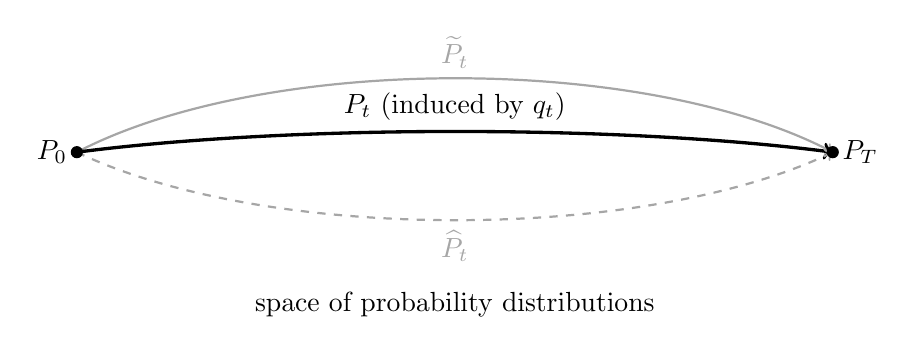
\begin{tikzpicture}[x=1cm,y=1cm]
    \coordinate (P0) at (0,0);
    \coordinate (PT) at (9.6,0);
    \draw[gray!70,thick,->]
      (P0) .. controls (2.4,1.25) and (7.2,1.25) ..
      node[pos=0.5,above,gray!70] {$\widetilde P_t$} (PT);
    \draw[black,very thick,->]
      (P0) .. controls (2.7,0.35) and (6.9,0.35) ..
      node[pos=0.5,above] {$P_t$ (induced by $q_t$)} (PT);
    \draw[gray!70,thick,dashed,->]
      (P0) .. controls (2.4,-1.15) and (7.2,-1.15) ..
      node[pos=0.5,below,gray!70] {$\widehat P_t$} (PT);
    \fill (P0) circle (2.2pt);
    \fill (PT) circle (2.2pt);
    \node[left] at (P0) {$P_0$};
    \node[right] at (PT) {$P_T$};
    \node[below] at (4.8,-1.65) {space of probability distributions};
\end{tikzpicture}
\end{document}
